\documentclass{article}
\usepackage{amsthm,amssymb,mathtools}
\usepackage{tikz}
\usetikzlibrary{graphs}

\usepackage{import}
\usepackage{xifthen}
\usepackage{pdfpages}
\usepackage{transparent}

\newcommand{\incfig}[2]{%
    \def\svgwidth{#2\columnwidth}
    \import{./figures/}{#1.pdf_tex}
}
\pdfsuppresswarningpagegroup=1


\newtheorem{theorem}{Theorem}
\newtheorem{definition}{Definition}
\newtheorem{lemma}{Lemma}
\newtheorem{corollary}{Corollary}
\newtheorem{remark}{Remark}
\newtheorem{proposition}{Proposition}
\newtheorem{example}{Example}

\newcommand{\lecture}[1]{\subsubsection*{#1}}
\begin{document}
\begin{theorem}[Eueler- Hierholzer Theorem]
	A graph $G$ is Eulerian, i.e., has a trail containing each edge exactly once, if and only if it is connected and each vertex has even degree.
\end{theorem}
\begin{proof}
	Assume that $G$ is connected and each of its vertices has even degree. We want to prove that it is Eulerian. We will use induction on the number $ \lvert E \rvert$ of edges in $G.$

	Let $m = 1.$ The only connected graphs having exactly one edge are $ G_1 =  ( \{v_1\}, \{\{v_1,v_1\}\} ),$ the graph with one vertex and a loop on it, and $G_2 = ( \{v_1, v_2\}, \{\{v_1,v_2\}\})$ the graph with two vertices and exactly one edge between them. The latter has vertices with odd degrees, so only consider $G_1.$
$G_1$ is Eulerian because the loop is a trail.

Let us assume that the statement is true for $ \lvert E \rvert = 1, \dotsc, k$ where $k \in \mathbb{N}$ is randomly chosen.
We now take a connected graph $G$ with $k+1$ edges such that every vertex has even degree.
By the preceeding lemma, $G$ contains a cycle $C$ because every vertex has degree $\geq 2.$
Let $G'$ be the graph obtained by removing this cycle form $G.$

Let $\tilde{G}$ be a connected component of $G'.$
Then $\tilde{G}$ is trivially connected, and for all vertives $v$ in $V(\tilde{G},$
the $\deg_{\tilde{G}}(v) = \deg{G'}(v),$ because no edge of $\tilde{G}$ connects to a
vertex outside it.
Thus, each vertex of $\tilde{G}$ is even and it satisfies the induction hypothesis.
It is thus Eulerian.

We proceed to construct an Eulerian walk on $G.$
Let $P = v_0, e_1, v_1, \dotsc, e_s, v_s$ be an Eulerian walk on a collection $ \mathcal{C}$
containing
the cycle $C$ and some or none of the connected components of $G'.$
If there is a vertex $v$ which is not in $P,$ then let $\tilde{G}$ be the connected component 
containing $v.$
There exists some $l \in \mathbb{N}$ such that $v_l \in \tilde{G}$ is contained in $P.$
This is because we assumed $G$ is connected and removed $C$ from it.
So, $v$ must have a path connecting it to $C,$ and it can only contain vertices
from $\tilde{G}$ and from $C$ as any vertex in this path is either in $P$ 
or in the same connected component as $v$ which is $\tilde{G}.$
As $C$ is non empty, $\tilde{G}$ has fewer than $k$ edges and has an Eulerian trail
by the induction hypothesis. Let this trail be 
$ v_l = x_0, e_1, x_1, e_2, x_2, \dotsc, e_r, x_r = v_l$
We then find that 
$  v_0, e_1, v_1, \dotsc, e_l,v_l = x_0, e_1, x_1, e_2, x_2, \dotsc, e_r, x_r = v_l, e_{l+1}, v_{l+1}, \dotsc, 
e_s = v_s = v_0$
is an Eulerian trail on $\mathcal{C} \cup \left\{ \tilde{G} \right\}.$

By induction, we have an Eulerian trail on $G.$

\end{proof}

\begin{definition}[Bipartite graphs]
	A graph $G = (V, E)$ is said to be bipartite if $V = A \cup  B$ with
	$ A \cap B = \phi,$ such that both $A$ and $B$ are independent sets.
	In this case, we call $A$ and $B$ the \emph{partitite} sets of $G.$
\end{definition}

We have the following characterisation of bipartite graphs.



\begin{theorem}[K\"onig]
	A graph $G$ is bipartite if and only if it has no odd cycles.
\end{theorem}

\begin{lemma}
	A graph is bipartite if and only if all its connected components are bipartite.
\end{lemma}

\begin{proof}	
	Given this lemma, we can prove the theorem by assuming that $G$ is connected.
\end{proof}

\lecture{Lecture - 09\hfil18 Sep 24, Wed}

\begin{definition}[Permutation]
	Let $S$ be a set. A function $ \sigma \colon S \to S$ is said to be a
	permutation on $S$ if it is a bijection.
\end{definition}

The set $ \Omega (S) $ of all the permutations on $S$ is a group when equipped with the
composition operation.
That is, for any $\sigma, \tau, \mu$ in $ \Omega(S),$ we have
$$ \sigma \circ ( \tau \circ \mu) = (\sigma \circ \tau) \circ \mu.$$
In other words, the composition operation is associative.
There exists the identity permutation $ \iota $ in $ \Omega(S)$
satisfying $\iota \circ \sigma = \sigma = \sigma \circ \iota$
for every $\iota$ in $ \Omega(S).$

The point $a \in S$ is said to be a fixed point of $ \sigma $ if $ \sigma(a) = a.$

The cycle $(a_1, a_2, \dotsc, a_k)$ denotes a permutation defined by:
$$ \sigma(a_1) = a_2, \sigma(a_2) = a_3, \dotsc, \sigma(a _{k-1} ) = a_k, \sigma(a_k) = a_1$$
and 
$$ \sigma(n) = n$$
for all $t $ in $S$ such that $t \not \in \{a_1, a_2, \dotsc, a_k\}.$

If $\sigma$ and $ \tau$ are disjoint cycles, that is,
$ \sigma =  (a_1, a_2, \dotsc, a_k)$ and $\tau = (b_1, b_2, \dotsc, b_l) $
and $a_i \not = b_j$ for any $i = 1, \dotsc, k $ or $ l =1 ,\dotsc, l,$
then $ \sigma \circ \tau = \tau \circ \sigma.$

\begin{definition}[$S_n$]
	The set of permutations on the set $\left[ n \right] = \left\{ 1, 2, \dotsc, n \right\} $ is denoted by $S_n.$
\end{definition}

\begin{theorem}
	Any permutation $ \sigma $ in $S_n$ can be written as a product of disjoint cycles.
	Moreover, this decomposition is unique upto reordering of the disjoint cycles.
\end{theorem}

\begin{proof}
	Consider the permutation $\sigma$ in $S_n.$
Since the fixed points of $\sigma$ do not appear in the cyclic decomposition of $\sigma,$
we induct on $m,$ the number of points in $ \left[ n \right] $ which are not fixed by $ \sigma.$
In other words, $ m = \lvert \left\{ a \in \left[ n \right] \, : \, \sigma(a) \not = a \right\}  \rvert .$
If $ m = 2,$ then there are exactly two points $a_1, a_2$ which are not fixed by $ \sigma.$
Then $\sigma = (a_1, a_2).$

Induction hypothesis:
Suppose every permutation $\sigma$ in $S_n$ with at most $k-1$ non fixed points
is a product of disjoint cycles.
We proceed to prove that $\sigma$ in $S_n$ is a product of disjoint cycles
if it has $m$ non-fixed points.
Pick a point $a_0$ in $ \left[ n \right] $ which is not a fixed point of $\sigma.$
We then examine the elements $$a_1 = \sigma(a_0), a_2 = \sigma^2(a_0), \dotsc, a_m = \sigma^m(a).$$
As these are all non fixed points of $\sigma,$ at least two of them are the same 
because these are $m+1$ in number and there are only $m$ non fixed points of 
$\sigma.$ Suppose $\sigma^j(a_0) = a_j = a_l = \sigma^l(a_0).$
If $j=0$ and $l=m,$ then 
$$ a_0, \sigma(a_0), \dotsc, \sigma^{m-1}(a_0) $$
is an $m$\nobreakdash-cycle.
Otherwise $ \tau = (a_j, a _{j+1}, \dotsc, a _{l-1})$ is a cycle with $l-1-j$
non fixed points.
For $s = \sigma(a_i),$ where $i=j, j+1, \dotsc l-1,$ we have
$$ \tau^{-1} \circ \sigma (s) = \tau^{-1}(\sigma^{i+1}(a_0)) = \sigma^i(a_0)$$
so that $\tau^{-1} \circ \sigma$ leaves $a_j, a _{j+1}, \dotsc, a_{l-1}$ fixed.
It also fixes all the points which are fixed by $ \sigma.$
Thus, it has $m - l + j < m $ non fixed points.
It can thus be expressed as a product of disjoint cycles.
$\tau$ is itself a cycle.
\end{proof}

\begin{proof}[Alternative proof]
Pick $a_1$ which is not a fixed point of $\sigma.$
If $\sigma^j(a) \not = a$ for $j = 1, \dotsc, m-1,$
then $\sigma = (a, \sigma(a), \sigma^2(a), \dotsc, \sigma^{m-1}(a) )$
is a cycle of length $m.$
If, otherwise, $\sigma^j(a) = a$ for some positive integer $j \leq m-1,$
we have $\sigma = \tau \circ \mu$ 
where $\tau(a) = \sigma(a)$ and $\tau^l(a) = \sigma^l(a)$
is a permutation which leaves all points other than those in
$T = \left\{ a, \sigma(a), \dotsc , \sigma^{j-1}(a) \right\} $
fixed and $\mu$ is the restriction of $\sigma$ to 
$\left[ n \right]  \setminus T.$
That is,
$$\mu(s) = \begin{cases}
	s, \quad & \text{ if } s \in T\\
	\sigma(s), \quad & \text{ otherwise }
\end{cases} $$
We know that $\tau$ fixes all points not in $S.$
We want to show that $\mu$ fixes all points in $S.$
Note that we can express $a = \sigma^j(a).$
If $\mu(b) = \sigma^i(a)$ for some element $\sigma^i(a)$ in $T,$
then $\mu(b) = \sigma(b),$ meaning that $b = \sigma^{i-1}(a) $ is in $T.$
However, this is not possible because $\mu$ is chosen to fix all points
in $T.$ We need to prove that $\mu$ is a permutation.
Given $t,r$ in $ \left[ n \right] ,$ we have
$ \mu(t) = t $ and $ \mu(r) = r$ if $r,t$ are in $T$
$ \mu(t) = \sigma(t) \not = \sigma(r) = \mu(r)$ if both $r$ ant $t$ are not in $T,$
and $ \mu(t) = \sigma(t) \not = r = \mu(r)$ if $r$ is in $T$ but $t$ is not in $T$
because $\sigma(t)$ is in not in $T.$
This shows that $\mu$ is injective.
Let $s$ be in $\left[ n \right].$ If $s = \sigma^i(a)$ for some positive integer $i \leq l,$
then $s $ is in $T$ and $s = \mu(s),$ otherwise $ s = \sigma(s') = \mu(s') $ for some $s'$ in
$ \left[ n \right] \setminus T$ because $ \sigma$ is surjective.
This shows that $ \mu$ is surjective.
Finally, we have that $ T = \left\{ a, \sigma(a), \dotsc, \sigma^{j-1}(a) \right\} $
has cardinality $j$ which is less than $m$ and so it leaves more than $n-m$ points fixed.



\end{proof}

\begin{theorem}[Decomposition into Transpositions]\label{thm:decomposition-into-transpositions}
	Any permutation $\sigma$ in $S_n$ can be written as a product of transpositions
	which may not be disjoint.
\end{theorem}

$$ 
\left( 
	\begin{array}{c}
		(a_{1,1} a_{1,2} \dotsc a_{1,n_1})\\
		(a_{2,1}  a_{2,2} \dotsc a_{2,n_2})\\
		\vdots \\
		(a_{k,1} a_{k,2} \dotsc a_{k,n_k}) 
	\end{array}
	\right)
	= \begin{array}{c}
		(a_{1,1} a_{1,2}) (a_{1,1} a_{1,3}) (a_{1,1} a_{1,4}) \cdots (a_{1,1} a_{1,n_1})\\
		(a_{2,1} a_{2,2}) (a_{2,1} a_{2,3}) (a_{2,1} a_{2,4}) \cdots (a_{2,1} a_{2,n_2}) \\
		 \vdots \\
		 (a_{k,1} a_{k,2}) (a_{k,1} a_{k,3}) (a_{k,1} a_{k,4}) \cdots (a_{k,1} a_{k,n_2}) \\
	\end{array}
	$$

\lecture{Lecture - 10 \hfill 20 Sep 2024}

\begin{definition}[Order of a permutation]
The order of a permutation $\sigma$ in $S_n$, denoted by $\operatorname{ord}(\sigma)$
is the smallest natural number $k$ such that $\sigma^k = \iota.$
\end{definition}

\begin{remark}
	For all $ \sigma$ in $S_n$ is at most $n!$ All of $ \sigma, \sigma^2, \dotsc, \sigma^{n!}$
	are distinct and cover all of $S_n$ so applying the Pigeonhole Principle, we know 
	that at least one of these should be $ \iota$ the identity permutation. This means
	$\operatorname{ \sigma} \leq n!.$ 
\end{remark}

\begin{remark}
	The order of the identity permutation $ \iota$ denoted by $\operatorname{ \iota} $
	is 1.
\end{remark}

\begin{corollary}[Order of product of disjoint cycles]
	Let $ \sigma = \tau_1 \, \tau_2 \, \cdots \, \tau_k$ where $ \tau_1, \tau_2, \dotsc
	\tau_k$ are disjoint cycles in $S_n.$ Then $\operatorname{ord}( \sigma) = 
	\operatorname{LCM}(k_1, k_2, \dotsc, k_k),$ where $k_i$ is the length of $ \tau_i$
	for each $i = 1, 2, \dotsc k.$
\end{corollary}

\section{Decomposition into transpositions}
Consider the polynomial $ \Delta_n$ in $n$ variables $x_1, x_2, \dotsc, x_n$ defined
by
$$ \Delta_n = \Pi _{1 \leq i < j \leq n} (x_i - x_j) $$

For any $ \sigma \in S_n,$ define the polynomial
$$ \Delta_n( \sigma) = \Pi _{1 \leq i < j \leq n} ( x _{\sigma(i) } - s _{ \sigma(j)} ). $$

Note that $ \Delta_n = \Delta( \epsilon) .$
Also, each factor in the expression of $ \Delta_n( \sigma) $ coincides with a factor of
$ \Delta $ but possibly introduces a $-$ sign.

\begin{definition}[Signature of a permutation]
	The signature of a permutation $ \sigma$ in $S_n$ is denoted by $\operatorname{sgn}
	( \sigma)$ and defined as
	$$ \operatorname{sgn}( \sigma) = \begin{cases}
	1 & \text{ if } \Delta_n(\sigma) = \Delta_n \\
	-1 & \text{ if } \Delta_n( \sigma) = - \Delta_n \\
	\end{cases}. $$
\end{definition}

\begin{theorem}
	For any natural number $ n \geq 2,$
	\begin{enumerate}
		\item If $ \sigma$ is a transposition, $ \operatorname{sgn} ( \sigma) = -1.$
		\item If $ \sigma, \tau$ are in $S_n,$ then $ \operatorname{sgn}( \sigma %
			\circ \tau) = \operatorname{sgn}( \sigma) \operatorname{sgn} ( \tau ) $
	\end{enumerate} 
\end{theorem}

\begin{proof}
	Let $ \sigma = (k \ l) $ is a transposition, then
	$$ \Delta_n( \sigma ) = \Pi _{1 \leq i < j \leq n} \left( x _{ \sigma(i) }
	 - x _{ \sigma(j)} \right).$$ 
	 I $i < j$ and $ \left\{ i, j  \right\}  \cap  \left\{ k,l \right\} = \phi,$
	 then $ x _{\sigma(i)} - x _{\sigma(j)} = x_i - x_j. $
	 We now consider the case that $ \left\{ i,j \right\} \cap \{ k, l \} \not = \phi.$
	 If $i < k ,$
	 then $x _i - x_ l $ becomes $x_i - x_k$ and $x_i - x_k$ becomes $x_i - x_l.$
	 If $j > l,$
	 $x_l - x_j$ becomes $x_k - x_j$ and
	 $x_k - x_j$ becomes $x_l - x_j.$
	 If $ k < i < l,$ $x_k - x_i$ becomes $x_l - x_i = -(x_i - x_l) $ 
	 and $ x_i  -x_l$ becomes $x_i - x_k = -(x_k - x_i).$
	Each of these changes does not affect $\Delta_n( \sigma).$
	 The only case which does, is if $i = k $ and $ j = l,$ then $ x_l - x_k$ becomes $x_k - x_l.$

	 Let $\sigma, \tau$ be in $S_n.$ Suppose $ \Delta_n( \tau)$ has exactly $r$ factors
	  of the form $x_j - x_i$ where $j > i,$ so that
	  $\operatorname{ ord} ( \sigma) = (-1) ^r.$ 
\end{proof}


\begin{definition}[Even and odd permutations]
	A permutation $ \sigma$ is said ot be even if, respectively.
	The set of all even permutations in $S_n$ is a subgroup of $S_n,$ i.e.,
	it is closed under product. It is called the alternating group of degree $n$
	and denoted by
	$$ A_n = \left\{  \sigma \in S_n \, : \; \operatorname{sgn}( \sigma) = 1 \right\}. $$
\end{definition}


\begin{remark}
	While we can write a given $ \sigma \in S_n$ as a product of transpositions in many different ways,
	what does not change is whether there are an odd or even number of transpositions.
\end{remark}


\section{Counting beyond permutations}

Recall that $\binom{n}{k},$ read ``$n$ choose $k,$"
and represents the number of ways in which a subset of $k$ objects 
may be chosen from a set of $n$ objects. It is also written as ${}^nC_k.$

\begin{definition}[$\binom{n}{k}$]
	For $n \in \mathbb{N},$ the \emph{binomial coefficient} $\binom{n}{k}$
	is the number of subsets of $[n]$ with $k$ elements.
\end{definition}

\begin{proposition}
	For $n$ in $\mathbb{N},$ we have $\binom{n}{k} =  \frac{n!}{k! (n-k)!}.$	
\end{proposition}


More egnerally, if $n$ is in $\mathbb{N},$ the number of partitions of $[n]$
with sizes $k_1, \dotsc, k_r$ is denoted by
$\begin{pmatrix} n \\ k_1 \: k_2\: \cdots \: k_r \end{pmatrix},$
and called a \emph{multinomial coefficient.}

\begin{theorem}
	For $n$ in $\mathbb{N}$ and $k_1, k_2, \dotsc, k_r$ in $\mathbb{N}$ such that
	$k_1 + k_ 2 + \cdots + k_r = n,$ we have 
	$$ \begin{pmatrix} n \\ k_1 \; k_ 2 \; \cdots \; k_r \end{pmatrix}
	= \frac{n!}{k_1 ! k_2 ! \cdots k_r!}. $$
\end{theorem}

\begin{theorem}[Binomial Theorem]
	If $n$ is in $\mathbb{N}$ and $x, y $ are elements in $\mathbb{R}$ (or in any ring 
	such that $xy = yx$), then 
	$$ (x+y)^n = \sum_{k=0}^{n} \binom{n}{k} x^k y^{n-k} .$$
\end{theorem}
Combinatorial Consequences


Settings $x=1, y=  1$ here, we get
$$
\sum_{j=0}^{n} \binom{n}{j} = (1+1)^n = 2^n.$$
Is there a bijective proof of this identity?

\section{Recurrence Relations}
\begin{example}[Fibonacci Numbers]
	The Fibonacci numbers are a sequence $\{ F_n \}_n$ of natural numbers defined by
	$$ F_1 = 1 \quad F_2 = 1 \\
	F_n = F_{n-2} + F_{n-1},$$
	for all natural numbers $n.$
\end{example}
This is a difference equation and may be viewd as an analogue of a differential
equation in a \emph{discrete time domain.}
So, a solution for $F_n$ for a general $n$ in $\mathbb{N}$ without
using recurrence relations may be though of as a solution to the difference equation.
The solution is $F_n = \frac{1}{\sqrt{5}} \left[ \left( 
\frac{1 + \sqrt{5}}{2}^n \right)  - \left( \frac{1 - \sqrt{5}}{2}^n \right) \right].$

\section{Power Series}
A \emph{Formal Power Series} is an expression of the form $ \sum_{n \in \mathbb{Z}^+}^{} 
a_n t^n,$ where $a_n$ is in $\mathbb{R}$ for each $n$ in $\mathbb{Z}^+.$


\noindent
\emph{Lecture -12 \hfill 25 Sep 2024, Wed}

\begin{definition}[Power series]
	A \emph{formal power series} over a field $\mathbb{K}$ in a variable $z$
	is an expression of the form
	$$ \sum_{n=0}^{\infty} a_n z^n,$$
	where $a_n$ is in $\mathbb{K}$ for each positive integer $n.$
\end{definition}
The set of all formal power series over $\mathbb{K}$ 
in a variable $t$ is denoted by $ \mathbb{K} [[t]]].$
A power series is distinct from a power series in that the latter is defined contigent
upon convergence.

\begin{definition}[Polynomial]
	A polynomial in a variable $t$ over a field $\mathbb{K}$ is an expression
	$$ f(t) = \sum{j=0}^{n} a_j t^j $$
	where $n$ is a fixed nonnegative integer and $a_n$ is in $\mathbb{K}$ for each integer $j \geq 0$ and $j \leq n.$
\end{definition}


The degree of a polynomial $f(t) = \sum_{j=0}^{n} a_n t^j$ is denoted as
$\deg(f(t)) = \max \left\{ m \; : \; a_m \not = 0 \right\}.$ The set of polynomials in $t$
with coefficients in $\mathbb{K}$ is denoted by $\mathbb{K} [t].$

Given a polynomial $f(t) = \sum_{j=0}^{n}  a_n t^n$ over $\mathbb{K}$ in $t,$ we can talk
about the associated polynomial function, which is independent of the variable $t.$
Call it $\overline{f}.$ It is defined as 
$$ \overline{f} (t) = \sum_{j=0}^{n} a_n t^n, \qquad \text{t } \in \mathbb{K} .$$
Defining an associated power series for a gievn formal power series needs more care
as it may not converge in $\mathbb{K}.$

Operations on $\mathbb{K} [[t]]$ include
\begin{enumerate}
	\item $ \left( \sum_{n=0}^{\infty} a_n t^n \right) 
	+ \left( \sum_{n=0}^{\infty} b_n t^n \right) 
	= \sum_{n=0}^{\infty} (a_n + b_n ) t^n.$
	\item$ \left( \sum_{n=0}^{\infty} a_n t^n \right) 
		\cdot \left( \sum_{n=0}^{\infty} b_n t^n \right) 
		 = \sum_{n=0}^{\infty} c_n t^n,$ 
		 where $c_n = \sum_{k=0}^{n} a_k b_{n-k}.$
\end{enumerate}
\begin{example}
	$$ \frac{1}{1-t} = \sum_{n=0}^{\infty}  t^n $$
	for $ \lvert t \rvert < 1.$
\end{example}

\begin{example}[Exponential power series]
	$$ e^t = \sum_{n=0}^{\infty} \frac{t^n}{n!} $$
	for all $t \in \mathbb{C}.$
\end{example}

\begin{example}[Derivative of a power series]
	given a power series $f(t) = \sum_{n=0}^{\infty} a_n t^n$ for $t \in \mathbb{C},$
	the derivative $f'$ is well defined with
	$f'(t) = \sum_{n=0}^{\infty} n a_n t^{n-1} .$
\end{example}




\noindent
\emph{Lecture -13 \hfill 27 Sep 2024, Fri}

Last time, we talked about recurrence relations, generating functions and formal power series.
For the Fibonacci sequence given by
$$ F_0 = 0, \quad F_1 = 1, \quad F_n = F_{n-1} + F_{n-2}, \forall \quad \text{integers} 
\quad n \geq 2,$$
we set $f(t) = \sum_{n \in \mathbb{N}}^{} F_n t^n$ and call it the \emph{Generating Function}
of this sequence.
Solving by substitution for $n=1,2,$ we get
\begin{align*}
	f(t) ={}& \sum_{n=1}^{\infty} F_n t^n \\
	={}& F_0 + t F_1 \sum_{n=3}^{\infty} F_{n-2} t^n + F_{n-2} t^n \\
	={}& t + (t + t^2) \sum_{n=1}^{\infty} F_{n} t^n \\
	={}& t + (t + t^2) f(t)
\end{align*}
The recurrence relation we get for it is
$$ f(t) =  \frac{t}{1 - t - t^2}.$$
Since $ 1 - t - t^2$ has roots 
$\alpha = \frac{1 + \sqrt{1 + 4}}{2} = \frac{1 + \sqrt{5}}{2}$ and 
$\beta = \frac{1 - \sqrt{1 +4 }}{2} = \frac{1 - \sqrt{5}}{2},$ 
we have
\begin{align*}
	( 1 - \alpha t)(1 - \beta t) ={}& 1 - (\alpha + \beta) t + \alpha \beta t^2\\
	={}& 1 - t - t^2 
\end{align*}
implying that
\begin{align*}
	f(t) ={}& \frac{t}{(1 - \alpha t ) ( 1 - \beta t)} \\
	={}& \frac{1}{\sqrt{5}} \left[  \frac{( \alpha - \beta ) t}{
	(1 - \alpha t)(1 - \beta t) }\right] \\
	={}& \frac{1}{ \sqrt{5}} \left[ \frac{1}{1 - \alpha t} - \frac{1}{ 1 - \beta t} \right].
\end{align*}
Recall that $ \frac{1}{1-s} = \sum_{n=1}^{\infty} s ^n$ for any real number $s.$
This allows us to write
\begin{align*}
	\sum_{n=1}^{\infty} F_n t^n ={}& \frac{1}{\sqrt{5}} \left[ \sum_{n=1}^{\infty} 
	(\alpha t)^n - \sum_{n=1}^{\infty} ( \beta t)^n \right] \\
	={}& \sum_{n=1}^{\infty} \frac{1}{\sqrt{5}} \left( \alpha^n - \beta^n \right) t^n.
\end{align*}
Therefore, $F_n = \frac{1}{\sqrt{5}} \left( \alpha^n  -\beta^n \right)$
from comparing the coefficients.

Since $ \lvert  \beta \rvert < 1,$ we get that $ \beta^n \to 0$ as $ n \to \infty.$
So $ \lvert  F_n - \frac{\alpha^n}{\sqrt{5}} \rvert \to 0$ as $n \to \infty.$
In other words $F_n \sim \frac{1}{\sqrt{5}} \alpha^n$ grows exponentially as $ \lvert 
\alpha\rvert >1.$

\section{Notation for approximations}
\begin{definition}[O notation]
	If $f,g$ are functions from $\mathbb{R}_+$ to itself, we say that $f(t) = O(g(t))$ if
	there exists finite real numbers $c, T$ such that $ f(t) \leq c g(t)$ whenever $ t > T.$
\end{definition}

\begin{definition}[O notation for sequences]
	Let $ \{ a_n \; : \; n \in \mathbb{N} \}$ be a sequence, and $ f\colon \mathbb{N} \to \mathbb{R}$ be a function. We say that $a_n = O(f(n))$ if there exists $ c $ in $\mathbb{R}$ and 
	$\mathbb{N}$ such that $ a_n \leq c f(n)$ for all $n $ in $\mathbb{N}$ whenever $n \geq N.$
\end{definition}
For example, $2^n = O(n!).$
\begin{definition}[Little `o' notation]
	Let $f \colon \mathbb{R}_+ \to \mathbb{R}_+.$
	We say that $f(t) = 0(g(t))$ if $\lim_{t \to \infty} \frac{f(t)}{g(t)} = 0,$
	that is $f(t)$ is growinf slower than $g(t).$
\end{definition}
\begin{example}
	We say that $a_n \sim f(n)$ if $\lim_{n \to \infty} \frac{a_n}{f(n)} = 1.$	
\end{example}
Note that $a_n = f(n) + o(f(n)) \Rightarrow a_n \sim f(n),$ if $\lim_{n \to \infty} 
f_n = \infty.$
\begin{theorem}[Stirling's Approximation]
	For any positive integer $n,$
	$$ n! \sim \sqrt{2 \pi n} \left( \frac{n}{e} \right)^n .$$
	In other words
	$$ \ln(n!) = n \ln \left( \frac{n}{e}  \right) - n + \frac{1}{2} \ln(n)
	+ \frac{1}{2} \ln(2 \pi ) + o(1).$$
\end{theorem}

\begin{remark}
	Note that
	\begin{align*}
		n ={}&  o(n \log (n)) \\
		\ln(n)={}& o(n) \\
		\frac{1}{2} \ln(2 \pi) ={}& o(\ln(n))\\
		o(1) ={}& \left( \frac{1}{2} \ln(2 \pi) \right)
	\end{align*}
	This means 
	$$ \ln(n!) = n \ln(n) + o(n \ln(n)) = (n \ln n)(1 + o(1))$$
	so that $\ln(n!) \sim n \ln n.$
\end{remark}

\begin{proof}[Sketch of proof]
	For any integer $n > 0,$ we have
	\begin{align*}
		\ln(n!) ={}& \sum_{i=1}^{n} \ln i \sim \int_1^n \ln x \mathrm{d} x.
	\end{align*}
	So,
\end{proof}



\noindent
\emph{Lecture - 14 \hfill 30 Sep 24, Mon}

\section{General Linear Recurrence Relations}

\begin{definition}[Linear Recurrence Relation]
	A \emph{recurrence relation,} or \emph{difference equation} is some relation constraining the elements of a sequence $\{ y_n \}_n.$
\end{definition}

A \emph{linear recurrence relation} on $\{ y_n \}$ is an equation
of the form 
$$ y_n = a_1 y_{n-1} + a_2 y_{n-2} + \cdots + a_k y_{n-k}.$$

\begin{remark}
	In order to find a recurrence relation involving $k$ terms, uniquely, we need
	initial conditions in the form of $k$ linearly independent
	equations, or equivalently, the first $k$ terms.
\end{remark}

Assuming that the $y_n$ is expressed by $x^n,$ for some each $n$ in 
$\mathbb{N},$ where $x$ is some value in $\mathbb{K},$
write the characteristic equation 
$$x^k = a_1 x^{k-1} + a_2 x^{k-2} + \cdots + a_{k-1} x + a_k.$$
Suppose the equation has $l$ distinct solutions $\alpha_1, \alpha_2,
\dotsc, \alpha_l,$ then any linear combination of these solutions:
$y^n = b_1 \alpha_1^n + b_2 \alpha_2^n + \cdots b_l \alpha_l^n$ is 
also a solution to the recurrence relation.
If the solutions $\alpha_1, \alpha_2, \dotsc, \alpha_l$ are not
distinct, and $\alpha_i$ is a solution of multiplicity $r$ where 
$r$ is some positive integer, then $\alpha_i^n, n \alpha_i^n, \dotsc,
n^{r-1} \alpha_i^n$ are all solutions of the recurrence relation.

\section{Catalan Numbers}
\begin{definition}[Curve]
	A \emph{curve} in a space $X$ is a continuous function $f \colon [0,1]
	\to X.$ 
\end{definition}
The points $f(0)$, respectively $f(1)$, as in the previous definition are known
as the starting point, respectively ending point, of $f.$
\begin{definition}[Simple Curve]
	A \emph{simple curve} is a continuous function $f \colon [0,1] \to X.$
	which is injective on $(0,1).$
\end{definition}
\begin{definition}[Closed curve]
	A \emph{closed curve} is a curve starting and ending at the same
	point.
\end{definition}
\begin{definition}[Jordan Curve]
	A Jordan curve is a simple closed curve in the plane $\mathbb{R}.$	
\end{definition}
\begin{theorem}[Jordan Curve Theorem]
	If $c$ is a Jordan curve in $\mathbb{R}^2$ then $\mathbb{R}^2
	\setminus \operatorname{Image}(c)$ consists of exactly 2 
	connected components, one bounded, called the `interior of $c$',	and one unbounded,
	called the `exterior of $c.$' The boundary of both of these connected components is $\operatorname{image}(c).$
\end{theorem}

\begin{definition}[Polygon]
	A polygon is a Jordan curve which is piecewise linear.
\end{definition}
\begin{definition}[Convex polygon]
	A convex polygon is a polygon whose interior is a convex set in
	$\mathbb{R}^2.$
\end{definition}

\incfig{polygons}{0.4}


$C_2 = 2,$ $C_3 = 5,$ $C_4 = 14,$ $C_5 = 42,$ $C_6 = 132,$ $C_7 = 429,$
$C_8 = 1430.$


\noindent
\emph{Lecture - 15 \hfill 02 Oct 24, Wed}

\begin{definition}[Catalan numbers]
	For any positige integer $n,$ the $n^\text{th}$ Catalan number
	denoted by $C_n$ is the number of ways of triangulating an
	$n$ sided polygon.
\end{definition}

\begin{figure}[h]
	\centering
	\incfig{triangulation-hexagon}{0.4}
	\caption{Triangulation of a hexagon}
	\label{fig:triangulation-hexagon}
\end{figure}

A triangulation of a polygon is a way of expressing the polygon as
a union of non self intersecting triangles.

The recurrence relation for Catalan numbers $C_n$ is 
$$C_{n+1} = \sum_{k=0}^{n} C_k C_{n-k}.$$
\begin{proof}
	Consider any triangulation of an $n+1$ sided polygon and fix one edge of it.
	
\end{proof}

This is a nonlinear recurrence relation. To solve it, set
$$ f(t) = \sum_{n=1}^{\infty} C_n t^n $$
to be the generating function of the Catalan numbers.
Note 
\begin{align*}
	\sum_{n=1}^{\infty} C_{n+1} t^n
	 ={}& \sum_{n=1}^{\infty} C_n t^{n-1} \\
	 ={}& \frac{1}{t} \left[ \sum_{n=0}^{\infty} C_n t^n - C_0 \right] \\
	 ={}& \frac{1}{t} \left[ F(t) - 1 \right].
\end{align*}
 Also,
 \begin{align*}
	 \sum_{n=1}^{\infty} C_{n+1} t^n
	 ={}& \sum_{k=0}^{\infty} i\left( C_k C_{n-k} \right) t^n \\
	 ={}& \sum_{n=1}^{\infty} \left( \sum_{k=0}^{n} C_k t^k C_{n-k}
	 t^{n-k}\right) \\
	 ={}& \sum_{n=1}^{\infty} \sum_{k=1}^{\infty} 
	 C_k t^k C_{n-k} t^{n-k} \chi_{[1,n]} (k) \\
	 ={}& \sum_{k=1}^{\infty} \sum_{n=1}^{\infty} 
	 C_k t^k C_{n-k} t^{n-k} \chi_{[1,n]} (k) \\
	 ={}& \sum_{k=1}^{\infty} C_k t^k
	 \left[ \sum_{n=1}^{\infty} C_{n-k} t^{n-k} \chi_{[1,n](k)} \right] \\
	 ={}& \sum_{k=1}^{\infty} C_k t^{k} \left[ 
	 \sum_{n=k}^{\infty} C_{n-k} t^{n-k} \right] \\
	 ={}& \sum_{k=1}^{\infty} C_k t^k
	 \left[ \sum_{n=0}^{\infty} C_n t^n \right]
 \end{align*}
 Multiplying the entire equation by $t,$ we get
 \begin{align*}
	 F(t) - 1
	 ={}& \sum_{n=2}^{\infty} C_{n} t^n\\
	 ={}& t \sum_{n=1}^{\infty} C_{n+1}t^n\\
	 ={}& t \sum_{k=1}^{\infty} C_n t^n \sum_{n=1}^{\infty} C_n t^n
	 \\
	 ={}& t F(t)^2
 \end{align*}

 This means $t F(t)^2 - F(t) +1 = 0.$
 This is a quadratic equation for $F(t).$
 Solving it gives us
 $$ F(t) = \frac{1 \pm \sqrt{1 - 4t}}{2t}. $$
 As we have $$ \sqrt{1 - 4t} =
 \sum_{n=1}^{\infty} \binom{1/2}{n} (-4t)^n
 = 1 - 2t - 2t^2 - 4t^3 - 10 t^4 - \cdots,
 $$ where $$ \binom{1/2}{n} = \frac{ \frac{1}{2} ( \frac{1}{2} - 1 )
\cdots ( \frac{1}{2} -n + 1)}{n!}.$$
Supopse 
$$ F(t) = \frac{1 - \sqrt{1 - 4t}}{2t}
 = \frac{1}{t} - 1 - t - 2t^2 - 5 t^3 - \cdots$$
Due to the $1/t$term, this is not a power series.
So we must have
\begin{align*}
	F(t) ={}& \frac{1 - \sqrt{4 - t}}{2t}\\
	={}& \frac{1 - 1 \sum_{n=1}^{\infty} \binom{1/2}{n} (-4t)^2}
	{2t} \\
	={}& \sum_{n=1}^{\infty}  - \frac{\binom{1/2}{n+1} (-4t)^{n+1}}{2} t^n.
\end{align*}

By comparing the terms of the power series, we get that
$$C_n = - \frac{\binom{1/2}{n+1} (-4)^{n+1} }{2} $$

\lecture{Lecture 16 \hfill 04 Oct 204, Fri}

\begin{definition}[Double Factorial]
	For any odd integer $n,$ we define the \emph{double factorial}
	$n!!$ of $n=2k-1$ by $1 \times 3 \times  5 \times \cdots 
	\times 2k-1.$
\end{definition}
For $n = 2k-1,$ we have
$$ n!! = \frac{(2k)!}{k! 2^k}.$$


\begin{lemma}
	For any positive integer $n,$ we have
	$$ \binom{1/2}{n+1} = 
	\frac{(-1)^n}{ (n+1) 2^{2n+1}} \binom{2n}{n}.$$
\end{lemma}

\begin{proof}
	Given a positive integer $n,$ we have
	\begin{align*}
		\binom{1/2}{n+1}
		={}& \frac{1/2 (1/2-1)\cdots(1/2-n)}{(n+1)!}\\
		={}& \frac{(1-2)(1-4)\cdots(1-2n)}{2^{n+1} (n+1)!} \\
		={}& \frac{(-1)^n}{2^{n+1} (n+1)!} (2n-1)!!\\
		={}& \frac{(-1)^n}{2^{n+1} (n+1)!} \frac{(2n)!}{2^n (n!}\\
		={}& \frac{(-1)^n}{(n+1) 2^{2n+1}} \frac{(2n)!}{(n!)^2}
	\end{align*}
	
\end{proof}


Using this expression for $\binom{1/2}{n},$ we can rephrase the 
expression for Catalan numbers in the following way.
$C_n$

\section{How does $C_n$ behave as $n$ gets large?}
From Stirling's Formula we know that
$n! \sim \sqrt{2 \pi n} \left( \frac{n}{e} \right) ^n.$ We can deduce
$$ \binom{2n }{n} = 
\frac{(2n)!}{(n!)^2} \sim
\frac{\sqrt{2\pi 2n} \left( \frac{2n}{e}^{2n} \right) }{ 2\pi n (
\frac{n}{e}^{2n}}.$$
which implies that
$\binom{2n}{n} \sim \frac{1}{\sqrt{\pi n}} 2^{2n}.$
Therefore
$$ C_n = \frac{1}{(n+1)} \binom{2n}{n}
\sim \frac{4^n}{(n+1) \sqrt{\pi n}}
\sim \frac{4^n}{ \pi n^{3/2}}.$$
In other words,
$\log_2 C_n = 2n - \frac{3}{2} \log_2 n - \frac{1}{2} \pi + o(1).$

\section{Aside: Another use for Cataln Numbers}
For any positive integer $n,$ $C_n$ also represents the number of ways
of breaking down the sum of $n+1$ numbers into pairwise operations.

For instance, when $n=2,$
$(x_1+  x_2) + x_3 = x_1  +(x_2 + x_3),$ and
when $n=3,$ 
$$(x_1 + x_2) + (x_3 + x_4) = (x_1 + (x_2 + x_3)) + x_4 $$
$$ = ((x_1 + x_2) + x_3) + x_4 = x_1 + (x_2 + (x_3 + x_4))$$
$$ = x_1 + (x_2 + x_3 ) +x_4 .$$

\section{Bell Numbers}
\begin{definition}
The $n^\text{th}$ \emph{Bell number $B_n$} is trhe number of partitions
of a set of $n$ elements.
\end{definition}

Recall that a partition of a set $A$ is a collection of nonempty
subsets $ \{ A_1, \dotsc, A_k\}$ such that 
$A_i \cap A_j =  \phi$ if $i \not = j$ and $\bigcup_{i \in [k]} A_i = A.$

\begin{example}
	$B_1 = 1$ because the only partition of $[1]$ is $\{\{1\}\}.$

	$B_2 = 2$ because the only partitions of $[2]$ are
	$\{ \{ 1,2\} \}$ and $\{ \{1\}, \{2\} \}.$

	$B_3 = 5$ because $\{ \{ 1\} , \{ 2, 3\} \},$ 
	$\{ \{1 \}, \{2\}, \{3\}\},$ $\{ \{ 1,2,3\}\},$
	$\{ \{1, 2\}, \{3\}\}$ and $\{ \{1,3\}, \{2\}\}$
	are the only partitions of $[3].$
\end{example}

\begin{lemma}
	For $n$ in $\mathbb{N},$
	$$ B_n = \sum_{k = 1}^{n} \binom{n-1}{k-1} B_{n-k}.$$
\end{lemma}

\begin{proof}
	In order for the formula to hold for $n=2,$ we need that	$2 = B_2 = \sum_{k=1}^{2} \binom{1}{k} B_k
	= \binom{1}{0} B_0 + \binom{1}{1} B_1
	= B_0 + B_1.$
	This means we need to set $B_0 = 1.$
	Suppose $ \{ A_1, A_2, \dotsc, A_k \}$ is a partition of $[n].$
	Then there is exactly one block, say $A_j$ which contains $n.$
	Then, $A_j = \{n\} \cup Y$ for some $ Y \subset [n-1].$
	If $ \lvert A_j \rvert = m,$ then $ \lvert Y \rvert = m-1;$ 
	so $Y$ could be one of $\binom{n-1}{m-1}$ subsets of $[n-1]$
	The remaining elements in $[n] \setminus A_j$ could be 
	partitioned in $B_{n-m}$ ways.
	Therefore,
	\begin{align*}
		B_n ={}&  \sum_{m=1}^{n} \binom{n-1}{m-1} B_{n-m}.
	\end{align*}
\end{proof}

This recurrence relaiton which we have obtained for $B_n$ is not 
a linear recurrence relation because the number of terms is not fixed
but grows with $n.$

\begin{definition}[Exponential generating function]
	Given a sequence $ \{ a_n\}_n,$ the \emph{exponential
	generating function} of $\{a_n\}_{n \in \mathbb{N}}$ is 
	$$ G(t) = \sum_{n1}^{\infty} \frac{a_n}{n!} t^n $$
\end{definition}

Consider the epxonential generating function of $\{B_n\}$
We have
\begin{align*}
	G(t) ={}& \sum_{n=0}^{\infty} \frac{B_n}{n!} t^n 
	\intertext{Differentiating it with respect to $t,$ we get}
	G'(t) ={}&  \sum_{n=1}^{\infty} \frac{b_n}{n!} n t^{n-1}\\
	={}& \sum_{n=1}^{\infty} \frac{B_n}{(n-1)!} t^{n-1} \\
	={}& \sum_{n=1}^{\infty} \frac{t^{n-1}}{(n-1)!}
	\sum_{k=1}^{n} \binom{n-1}{k-1} B_{n-k} \\
	={}& \sum_{n=1}^{\infty} \sum_{k=1}^{n} 
	\frac{t^{k-1}}{(k-1)!} \frac{B_{n-k} t^{n-k}}{(n-k)!} \\
	={}& \sum_{n=1}^{\infty} \sum_{k=1}^{\infty} 
	\frac{t^{k-1}}{(k-1)!} \frac{B_{n-k} t^{n-k}}{(n-k)!}
	\chi_{[1,n]}(k) \\
	={}& \sum_{k=1}^{\infty} \sum_{n=1}^{\infty}
	\frac{t^{k-1}}{(k-1)!} \frac{B_{n-k} t^{n-k}}{(n-k)!}
	\chi_{[1,n]}(k) \\
	={}& \sum_{k=1}^{\infty} \frac{t^{k-1}}{(k-1)!}
	\sum_{n=k}^{\infty} \frac{t^{n-k}}{(n-k)!} B_{n-k} \\
	\intertext{Replacing $n$ with $n+k$, we get}
	={}& \sum_{k=0}^{\infty} \frac{t^k}{k!}
	\sum_{n=0}^{\infty} \frac{t^n}{n!} B_n\\
	={}& \left( \sum_{k=0}^{\infty} \frac{t^k}{k!} \right) 
	\left( \sum_{n=0}^{\infty} \frac{t^n}{n!} B_n \right) \\
	={}& e^t G(t).
\end{align*}

Therefore, $G'(t) = e^t G(t)$ which means
$$[\log G(t)] ' = \frac{G'(t)}{G(t)} = e^t.$$
So, $$\log G(t) = e^t + k,$$
where $k$ is some constant in $\mathbb{R}.$
This means $G(t) = A e^{e^t},$ where $A$ is some positive number.
We had that $G(0) = B(0) = 1.$  So, $A e^1 = 1$
and $A = \frac{1}{e}.$
This means $$G(t) = e^{e^t - 1}.$$


\lecture{Lecture - 17\hfill 07 Oct 24, Mon}

\section{The Inclusion-Exclusion Principle}
The simplest possible manifestation of the inclusion exclusion Principle
is
$$ \lvert A \cap B \rvert = \lvert A \rvert + \lvert B \rvert - \lvert A \cap B \rvert$$
for any two finite substes $A$ and $B$ of a set $X.$

\begin{theorem}
	Let $A$ be a finite set, and $A_1, A_2, \dotsc A_k \subseteq A.$
	Then
	$$ \lvert A \setminus \bigcup_{j \in [k]} A_j \rvert
	= \sum_{J \subseteq[k]} (-1)^{ \lvert  J \rvert} \lvert A_J \rvert$$
	where $A_J = \bigcap_{j \in J} A_j,$ and $A_{\phi} = A.$
\end{theorem}

\begin{remark}
	We can think of $A_1, A_2, \dotsc, A_k$ as a bunch of bad sets
	which we want to exclude from $A.$
\end{remark}

\begin{proof}[My Proof]
	Let $S_a = \{ i \in [n] \, : \, a \in A_i \}$ for each $a$ in 
	$A.$ Let $B = \bigcup_{i \in [n]} A_i.$ We may write
\begin{align*}
	\lvert B \rvert% 
	={}& \sum_{a \in B} 1 \\
	={}& \sum_{a \in B} 1 - (1-1)^{ \lvert S_a \rvert} \\
	\intertext{(because $ \lvert S_a \rvert \not = 0$ for $a$
	in $B.$)}
	={}& \sum_{a \in B} \sum_{j=1}^{ \lvert S_a \rvert} (-1)^j
	\binom{ \lvert S_a \rvert}{j} \\
	={}& \sum_{a \in B} \sum_{j=1}^{ \lvert S_a \rvert} (-1)^j
\sum_{\substack{ J \subseteq [S_a]\\ \lvert J \rvert = j}} 1 \\
	\intertext{(the binomial coefficient is simply the number of ways of choosing $j$ sized subsets from $S_a.$)}
	={}& \sum_{a \in B} \sum_{j=1}^{ \lvert S_a \rvert}
\sum_{\substack{ J \subseteq [S_a]\\ \lvert J \rvert = j}} (-1)^{ \lvert J \rvert} \\
	={}& \sum_{a \in B} \sum_{J \subseteq [S_a]} (-1)^{ \lvert J \rvert} \\ 
	={}& \sum_{a \in b} \sum_{J \subseteq [n]} (-1)^{ \lvert J \rvert} \prod_{i \in J} \chi_i(a) \\
	\intertext{(because the product $\prod_{i \in J} \chi_i(a) $
		is $1$ if $a$ is in $\bigcap_{i \in J} A_i$ and
	$0$ otherwise)}
	={}& \sum_{J \subseteq [n]} (-1)^{ \lvert J \rvert}
	\sum_{a \in B} \chi_1(a) \cdots \chi_n(a) \\
	\intertext{(because finite double summations can be interchanged.)}
	={}& \sum_{J \subseteq [n]} (-1)^{ \lvert J \rvert}
	\lvert \bigcap_{j \in J} A_j \rvert .
\end{align*}
\end{proof}

\iffalse
\begin{proof}
	The right hand side of the equation may be rewritten as
\begin{align*}
	& \sum_{m=0}^{k} (-1)^m \sum_{\substack{J \subseteq [k] \\ \lvert J \rvert = m}} \lvert A_J \rvert \\
	={}& \sum_{m=0}^{k} \sum_{\substack{J \subseteq[k] \\
	\lvert J \rvert = m}} \chi_J(i)
\end{align*}
Fix $a$ in $A.$
Then
\begin{align*}
	={}& \sum_{\substack{ J \subseteq [k] } (-1)^{ \lvert J \rvert}}
		\chi_{A_J} (a) \\
	& \sum_{\substack{ J \subseteq [k]\\ a \in A_J }} \chi_{A_J} (a) \\
	={}& \sum_{J \subseteq S_i} (-1)^{ \lvert J \rvert},
\end{align*}
 where $S_i = \{ j \in [k] \,:\, a \in A_j \}.$
 If $S_i \not = \phi,$ then $ \sum_{J \subseteq [k]} (-1)^{ \lvert J \rvert} \chi_{J}(i) = (-1)^0 \chi_{A_\phi}(a) = 1.$
 If $S_i \not = \phi,$ then
 \begin{align*}
	& \sum_{J \subseteq [j]} (-1)^{ \lvert J \rvert } \chi_{A_J} (i)\\
	={}& \sum_{J \subseteq [S_i] } (-1)^{  }\\
	={}& \sum_{j=0}^{ \lvert S_i \rvert} (-1)^i \sum_{
	\substack{ J \subseteq [k] \\ \lvert J \rvert = j}} 1 \\
	={}& d
 \end{align*}
\end{proof}

\fi


\noindent
\emph{Lecture - 18\hfill 09 Oct 24, Wed}

\begin{definition}[Derangements]
	If $n$ in $\mathbb{N}$ is a positive integer and $\sigma \colon [n] \to [n]$ is a permutation of $[n],$ i.e., $\sigma \in S_n,$ such that
	$\sigma(i) \not = i,$ for any $i in $ $[n],$ then $\sigma$
	is said to be a derangement of $[n].$
\end{definition}
\begin{theorem}
	If $d_n$ is the number of derangements of $[n],$ then
	$$ d_n = \sum_{j=0}^{n}  (-1)^j \binom{n}{j} (n-j)!
	= \sum_{j=0}^{n} (-1)^j \frac{n!}{j!} $$
\end{theorem}

\begin{remark}
	$\sum_{j=0}^{n} \frac{(-1)^j}{j!} $ is an approximation for 
	$ \frac{1}{e}.$
\end{remark}

\begin{proof}
	Let $A = S_n$ and $A_i$ be the set of all permutations $\sigma$
	in $S_n$ such that $\sigma)i) = i.$ So, according to  the Inclusion Exclusion Principle, the number of permutations which do not fix any elements at all, $d_n,$ is
	\begin{align*}
		d_n = {}& \lvert A \setminus \bigcup_{i \in [n]} A_i \rvert \\
		={}& \sum_{J \subseteq [n]} (-1)^{ \lvert J \rvert} 
		\left( \lvert A_J \rvert \right) \\
		={}& \sum_{J \subseteq [n]} (-1)^{ \lvert J \rvert} 
		(n - \lvert J \rvert )!\\
		={}& \sum_{j=0}^{n} (-1)^j \binom{n}{j} (n-j)!
	\end{align*}
\end{proof}

This theorem has a nice probabilistic interpretation.
Suppose we have a large number $n$ of individuals in a room who put their 
umbrellas down at the door when they come in. If each person randomly picks up an umbrella while leaving, then the probability that no person gets their umbrella back is $ \frac{d_n}{n!}$ which tends to $ \frac{1}{e}$ as $n \to \infty.$

\begin{theorem}[Counting Surjective maps]
	The number of surjective maps from $[n]$ to $[k]$ is 
	$$ \sum_{j=0}^{k} (-1)^j \binom{k}{j} (k-j)^n.$$
\end{theorem}

\begin{proof}
Let $A_i = \left\{ f \colon [n] \to [k] \; \middle| \;
f(j) \not =  i \, \forall \, j \in [n] \right\}.$
So, $ \lvert A_i \rvert = (k - \lvert A_j \rvert )^n.$
By Inclusion Exclusion Principle, we get that the cardinality of $S$, 
the set of all surjective functions from $[n]$ to $[k].$
\begin{align*}
	\lvert S \rvert ={}& \sum_{J \subseteq [k]} (-1)^{ \lvert J \rvert} \lvert A_J \rvert \\
	={}& \sum_{j=0}^{n} (-1)^j \sum_{\substack{J \subseteq [k] \\
\lvert J \rvert = j }} (k - j)^n \\
	={}& \sum_{j=0}^{n} (-1)^j \binom{k}{j} (k-j)^n.
\end{align*}
\end{proof}


\section{Stirling numbers of the first kind}
Recall that we hada  factorization of permutations as a product of disjoint cucles (unique upto obvious invariances).
The unsigned Stirling number of the first kind 
are 
$$ \begin{bmatrix} n\\k \end{bmatrix} $$
which is the number of permutations of $[n]$ which can be written as a product of $k$ disjoint cycles, over positive integers $n,k$ such that $k \leq n .$
The \emph{Signed Stirling numbers of the first kind are} $$s(n,k) = (-1)^{n-k} \begin{bmatrix} n\\k \end{bmatrix} , $$
where $k \leq n$ are positive integers.

Note $s(n,n) = 1$ because only the identity permuatation on $[n]$ can be written as a product of $n$ disjoint cycles. Observe that
$$ \sum_{j=1}^{n}  \begin{bmatrix} n \\ k \end{bmatrix} 
= \lvert S_n \rvert = n!. $$

\begin{theorem}
	If $n \geq k$ are positive integers, then 
	$$ s(n+1, k) = - n \times s(n,k) + s(n, k-1). $$
\end{theorem}

\begin{proof}
Consider $$S_{n,k} = \left\{ \sigma \in S_n \; : \;
\sigma \text{ can be written as a product of }
k \text{ disjoint cycles } \right\}, $$
and write $S_{n+1, k} = A \cup B,$ where
$A = \left\{ \sigma \in S_{n+1, k}  \, : \, \sigma(n+1) = n+1 \right\} .$
We may write $ \lvert A \rvert = \begin{bmatrix} n \\ k-1 \end{bmatrix} = (-1)^{n-k+1} s(n, k-1) .$
Given an element $ \sigma$ in $S_{n+1,k} \setminus A,$ we observe that
$\sigma$ has $k$ cycles in its decomposition. So, we can write $l= 
\sigma(n+1).$ Then $\sigma \circ (n+1 \; l)$ is in $S_{n,k}.$
Conversely, if $\sigma \in S_{n,k}$ then for any $l$ in $[n],$
$\sigma \circ (l \, n+1)$ is in $S_{n+1,k}.$
To make this observation more ludic, we can write any element of $ \lvert S_{n+1,k} \setminus A \rvert $ 
as $\sigma = \sigma_1 \sigma_2 \cdots \sigma_k,$ where $\sigma_i$ is 
a cycle for each $i$ in $[k]$ and $\sigma_i, \sigma_j$ are disjoint for
disjoint $i,j$ in $k].$ Let $l = \sigma^{-1}(n+1)$ and $i$ be
the unique element in $[k]$ such that $\sigma_i(l) = n+1.$
This uniqueness follows from the disjointness of the cycles.
So, we may write 
\begin{align*}
	\sigma ={}& \sigma_1 \cdots \sigma_{i-1} (a_1 \, a_2 \, \dotsc l \, n+1) \sigma_{i+1} \cdots \sigma_n \\
	={}& \sigma_1 \cdots \sigma_{i-1} (a_1 \, a_2 \, \dotsc l ) (l \, n+1) \sigma_{i+1} \cdots \sigma_n \\
	={}& \sigma_1 \cdots \sigma_{i-1} (a_1 \, a_2 \, \dotsc l ) \sigma_{i+1} \cdots \sigma_n (l \, n+1).
\end{align*}
Here,  $\sigma_1 \cdots \sigma_{i-1} (a_1 \, a_2 \, \dotsc l ) \sigma_{i+1} \cdots \sigma_n $ is in $S_{n,k}.$
The number of elements in $S_{n+1,k}$ is $-s(n,k)$ and each element in 
$S(n,k)$ corresponds to $n$ distinct elements in $S(n+1,k)$ arising from $n$ distinct choices of the image $\sigma^{-1}(n+1) = l.$
\end{proof}

\lecture{Lecture - 19\hfill 11 Oct 24, Fri}

\begin{definition}[The falling factorial]
	For any positive integer $n,$ we wdefine the \emph{falling factorial} to be 
	$$ (t)_n = t(t-1) \cdots (t - n+1).$$
\end{definition}


\begin{definition}[The rising factorial]
	For any positive integer $n,$ we define the \emph{rising factorial} to be 
	$$ t^{(n)} = t(t+1) \cdots (t + n-1).$$
\end{definition}


\begin{remark}
	$$\binom{ \alpha } {n} = \frac{( \alpha)_n}{n!} $$
\end{remark}

\begin{remark}
	$ t^{(n)} = (-1)^n (-t)_n $
\end{remark}


\begin{theorem}
	For any $t$ in $\mathbb{R}$ and any $n $ in $\mathbb{N},$ we have
	$$(t)_n = \sum_{k \in [n]} s(n,k) t^k. $$
\end{theorem}

\begin{remark}
	For fixed $n$ in $\mathbb{N},$ the generating function of 
	$\left\{ s_{n,k} \;:\; k \in \mathbb{N} , k \leq n \right\} $ is
	$$ (t)_n = \sum_{k \in [n]} s(n,k)t^k. $$
\end{remark}
\begin{proof}
	For $n=1,$ $s(1,1) = 
	\begin{bmatrix} 1\\1 \end{bmatrix}.$
Suppose the formula is true for some $n$ in $\mathbb{N}.$ Then,
\begin{align*}
	(t)_{n+1}
	={}& (t-n) (t)_n \\
	={}& (t-n) \left( \sum_{k \in [n]} s(n,k) t^k \right)  \\
	={}& \sum_{k \in [n]} s(n,k) t^{k+1} - n \sum_{k \in [n]} s(n,k) t^k  \\
	={}& \sum_{k=0}^{n-1} s(n,k-1) t^k - \sum_{k=0}^{n} n s(n,k) t^k\\
	={}& 0 + \sum_{k=1}^{n-1}  s(n,k-1) t^k - \sum_{k=0}^{n-1} n 
	s(n,k) t^k - n s(n,n) \\
	={}& \sum_{k=1}^{n-1} s(n+1,k) t^k + (-1)^{n-k+1} (n-1)! \times n t^{n+1}\\
	={}& \sum_{k=0}{n} s(n+1,k) t^k.
\end{align*}
\end{proof}



\section{Stirling Numbers of the Second Kind}

\begin{definition}
	The Stirling numbers of the second kind are denoted as 
	$$ \begin{Bmatrix} n\\k \end{Bmatrix} = S(n,k)$$
	for positive integers $n,k$ and they represent the
	number of partitions of $[n]$ into $k$ nonempty blocks.
\end{definition}


\begin{remark}
	As the $n^\text{th}$ Bell number $B_n$ is the number of partitions is the toal number of partitions of $[n]$ into nonempty blocks, we have
	$$B_n = \sum_{k=1}^{n} \begin{Bmatrix} b\\k\end{Bmatrix}.$$ 
\end{remark}



Any partition of $[n]$ into $k$ nonempty blocks is related to the
surjective functions from $[n]$ to $[k].$ Given a surjective function
$f \colon [n] \to [k],$ the sets $\{ f^{-1}(1), \dotsc, f^{-1}(k)\}$
form a partition of $[n]$ into $k$ non empty blocks.

Conversely, given a partition $A_1, A_2, \dotsc, A_k$ of $[n]$ into $k$ nonempty blocks and $\sigma$ in $S_k,$ $f \colon [n] \to [k]$ defined by
$f(i) = \sigma(j)$ such that $i$ is in $A_{j}$ is a surjective function.
Thus, we have proved the following theorem
\begin{theorem}
	If $n \geq k,$ then the number of surjective maps from
	$[n]$ to $[k]$ is expressed by the following relation
	\begin{align*}
		k! \begin{Bmatrix} n\\k\end{Bmatrix}
		={}& \lvert \{ f\colon [n] \to [k] \; | \;
		f \text{ is surjective } \} \rvert \\
		={}& \sum_{j=0}^{k} (-1)^j \binom{k}{j} (k-j)^n.
	\end{align*}
\end{theorem}


\begin{remark}
	We have the recurrence relation for positive integers $k \leq n,$
	$$ \begin{Bmatrix} n\\k\end{Bmatrix} = 
	\begin{Bmatrix}n-1\\k-1 \end{Bmatrix} + 
	k \begin{Bmatrix}n-1\\k-1 \end{Bmatrix}. $$
\end{remark}


\begin{theorem}
for any $t$ in $\mathbb{R},$ and any $n$ in $\mathbb{N},$ we have
$$	 t^n = \sum_{k \in [n]} 
\begin{Bmatrix} n\\k \end{Bmatrix} (t)_k. $$
\end{theorem}

\begin{proof}
	Assuming that $$t^{k} = \sum_{i \in [k]} 
	\begin{Bmatrix} n \\ i \end{Bmatrix} (t)_i,$$
\begin{align*}
	t^{k+1} ={}& (t-k) t^k + k t^k \\
	={}& COMPLETE THIS!
\end{align*}
\end{proof}

\begin{definition}
	A vector space $V$ over a field $\mathbb{F},$ is a set
	$A$ equipped with two operations $+ \colon A \times A \to V$ usually called `addition' and
	$\ \cdot \  \colon \mathbb{F} \times A \to A$ called the `scalar multiplication' such that for any $\alpha, \beta$ in
	$\mathbb{F}$ and $x,y$ and $z$ in $A,$
	\begin{enumerate}
		\item $\alpha(\beta x) = (\alpha \beta)x,$
		\item $(\alpha + \beta) x = \alpha x + \beta x,$
		\item $\alpha(x + y) = \alpha x + \alpha y,$
		\item $(\alpha + \beta) x = \alpha x + \beta x,$
		\item $ 1 x = x,$
		\item $x+y = y+x,$
		\item $(x+y)+z = x + (y+z),$
	\end{enumerate}
	where $1$ and $0$ are the multiplicative and additive identity of $\mathbb{F}$ and there exists $\mathbf{0}$ in $A$ such that $0 x = \mathbf{0}$
	for all $x$ in $A.$
\end{definition}

Hereafter, for a vector space $V,$ the underlying set $A$ will also be 
represented by $V.$

The vector space of polynomials over an unkown $t$ with coefficients
in $\mathbb{F},$ is a vector space over $\mathbb{F}.$

Let $\mathcal{P}_n$ be the (sub)space of all polynomials in
$\mathbb{F}[t]$ of degree at most $n.$ Then  
the dimension of $\mathcal{P}_n$ is $n+1$ because $\{ 1, t, t^2,
\dotsc, t^n \}$ forms a basis of it.

Note that $\{ (t)_0, (t)_1, \dotsc, (t)_n \}$ and 
$\{ t^{(0)}, t^{(1)}, \dotsc, t^{(n)} \}$ form two separate bases of 
$\mathcal{P}_n.$ The change of basis formulae for these bases are given
by the relation between $(t)_i$ and  $t^{(i)}.$

If $A = \{ s(i,j) \}$ and $ B = \{S(i,j) \} $ are $n \, \times  \, n$
matrices, then $A = B^{-1}.$

The convention is to write 
$$\begin{bmatrix}n\\0\end{bmatrix} =
\begin{Bmatrix}n\\0\end{Bmatrix} = 
\begin{cases}
0 & \text{ if } n \in \mathbb{N} \\
1 & \text{ if } n = 0 \\
\end{cases}. $$


\lecture{Lecture - 20\hfill 14 Oct 2024, Mon}

Note that $\{1 = t^0, t, t^2, \dotsc, t^n\} = \mathcal{B},$
$\{(t)_0, (t)_1, (t)_2, \dotsc, (t)_n \} = \mathcal{C},$ and
$\{t^{(0)}, t^{(1)}, t^{(2)}, \dotsc t^{(n)}\} \- = \mathcal{D}$
form three separate bases of $\mathcal{P}_n.$



So, the formula
\begin{align*}
	t^n ={}& \sum_{k \in [n]}^{} \begin{Bmatrix} n\\k \end{Bmatrix} t^k \\
	={}& 
\end{align*}


\begin{theorem}
	If $\{ f_n \}$ and $\{g_n\}$ are sequences related by
	$$ g_n = \sum_{k=a}^{n}  \begin{Bmatrix} n\\k \end{Bmatrix} f_k,
	\qquad \forall \/ n \geq a,$$
	then we have the inversion formula
	$$ f_n = \sum_{k=a}^{n} \begin{bmatrix} n \\k \end{bmatrix}
	(-1)^{n-k} g_k, \qquad \forall \/ n \geq a.$$
\end{theorem}

\begin{remark}
	If $a=0,$ or $1,$ this follows immediately from the fact that
	$B = A^{-1}.$ Note that if $a=0,$ for $n=0,$ we have $f_0 = g_0,$
	and for $n=1,$ would imply 
	$$g_1 = \begin{Bmatrix}1\\1\end{Bmatrix} f_1, \quad
	f_1 = \begin{Bmatrix}1\\1\end{Bmatrix} g_1.$$
\end{remark}

\subsubsection*{An application to calculus}
It is easier to compute the differences between functions rather than
to compute the derivatives. In this case, we choose to approximate the
interval by a grid. A real analytic function is a smooth i.e.,
infinitely differentiable function for which the infinite Taylor Series converges about any point. For a real analytic function, $f \colon \mathbb{R} \to \mathbb{R},$ we have
\begin{align*}
	f(x+y) - f(x) ={}& y f'(x) + \frac{f^{(2)}}{2!} y^2 + \frac{f^{(3)}}{3!} y^3 + 
	\cdots\\
	={}& \sum_{k=1}^{\infty} \frac{y^k}{k!} f^{(k)}(x).
\end{align*}

In particular, if $\Delta$ represents the finite difference operator,
given by
$$(\Delta f)(x) = f(x+1) - f(x),$$
then
$$ (\Delta f)(x) = \sum_{k=1}^{\infty} \frac{f^(k)(x)}{k!} .$$


More generally, we can talk about the higher order finite difference operators such as
\begin{align*}
	( \Delta^2 f)(f) ={}& (\Delta(\Delta f))(x) \\
	={}& \Delta \left[ f(x+1) - f(x) \right] \\
	={}& \left[ f(x+2) - f(x+1) \right] - \left[ f(x+1) - f(x) \right] \\
	={}& f(x+1) - 2 f(x+1) + f(x).
\end{align*}
Similarly, we define $(\Delta^k f)(x) = (\Delta (\Delta^{k-1} f)) (x).$
\begin{theorem}
	If $f$ is real anlaytic, then
	$$ \frac{1}{k!} (\Delta ^k f)(x) = \sum_{n=k}^{\infty} 
	\frac{S(n,k)}{n!} f^{(n)} (x) .$$
	Consequently,
	$$ \frac{1}{k!} f^{(k)} (x) = \sum_{n=k}^{\infty} $$
	FILL THIS
\end{theorem}


\section{Graphs}
\begin{definition}[Adjacency Matrix]
	Given a graph $G = (V,E),$ we define its \emph{adjacency matrix} $A,$ as a matrix with rows and columns indexed by $V,$ such that
	$A(x,y)$ is the number of edges from $x$ to $y.$
\end{definition}

\begin{example}
	For the graph
	\begin{figure}[h]
	\centering
		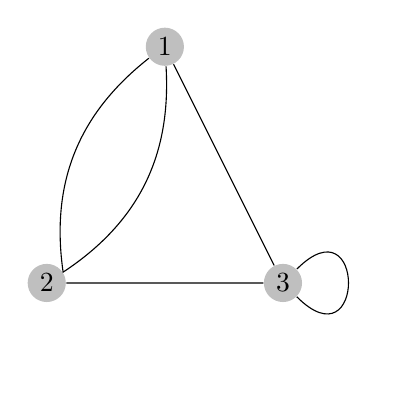
\begin{tikzpicture}
			\tikzstyle{vertex}=[circle,fill=black!25,minimum size=12pt,inner sep=2pt]
			\node[vertex] (g_1) at (3,3) {1};
			\node[vertex] (g_2) at (1.5,0) {2};
			\node[vertex] (g_3) at (4.5,0) {3};
			\draw (g_1)  to [bend left] (g_2) to [bend left]  (g_1) (g_2) -- (g_3) -- (g_1) (g_3) to [out=45, in = -45, looseness=9] (g_3);
		\end{tikzpicture}
	\end{figure}
	We have the adjacency matrix
	$\begin{bmatrix}
		0&2&1\\
		2&0&1\\
		1&1&2
	\end{bmatrix} .$
\end{example}

\begin{theorem}
	Let $G = (V,E)$ be a graph without loops and with adjacency matrix $A.$ For $x,y$ in $V,$ and any $l$ in $\mathbb{N},$ 
	$A^l(x,y)$ is the number of $(x,y)$ walks of length $l$ in $G.$
\end{theorem}

Here, $A^l(x,y)$ represents the $(x,y)^{\text{th}}$ entry of the matrix $A^l.$

\begin{figure}[h]
\centering
	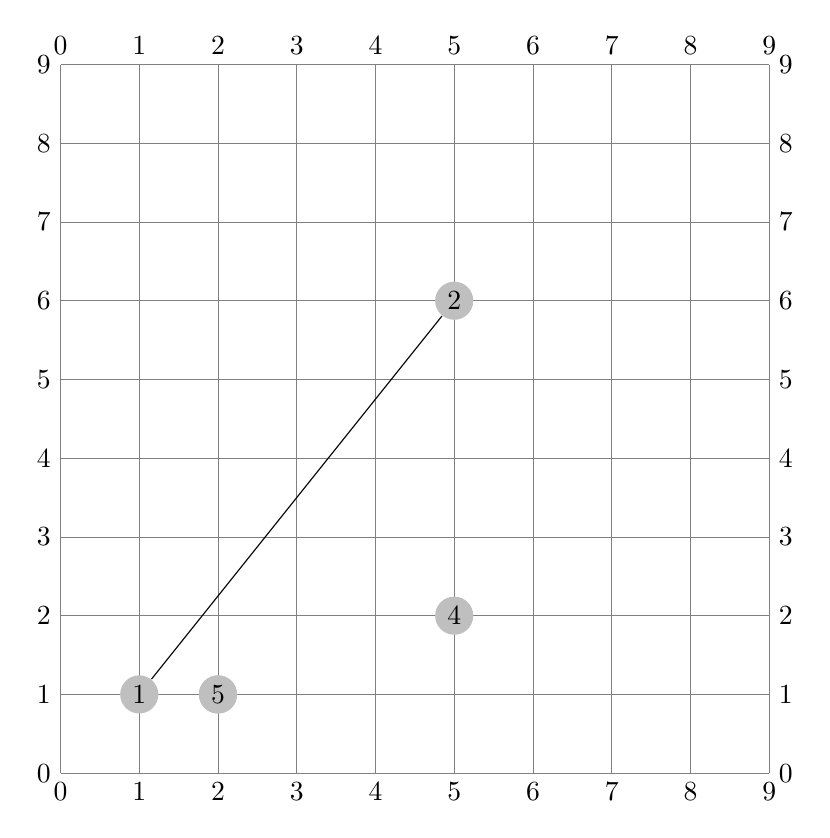
\begin{tikzpicture}
		\draw[help lines] (0,0) grid (9,9);
		\foreach \x in {0,...,9}{
			\draw(0,\x) node[anchor=east]{\x};
			\draw(9,\x) node[anchor=west]{\x};
			\draw(\x,0) node[anchor=north]{\x};
			\draw(\x,9) node[anchor=south]{\x};
		}
		\tikzstyle{vertex}=[circle,fill=black!25,minimum size=12pt,inner sep=2pt]
		\node[vertex] (g_1) at (1,1) {1};
		\node[vertex] (g_2) at (5,6) {2};
		\node[vertex] (g_3) at (2,1) {3};
		\node[vertex] (g_4) at (5,2) {4};
		\node[vertex] (g_5) at (2,1) {5};
		\draw (g_1) -- (g_2);
	\end{tikzpicture}
\end{figure}


\begin{figure}[h]
\centering
	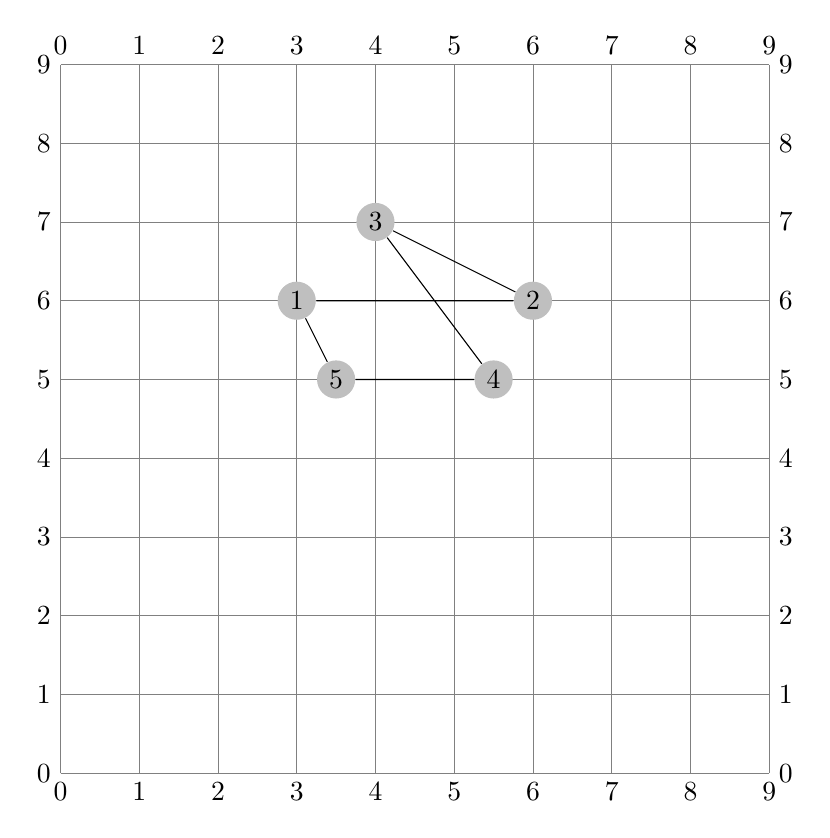
\begin{tikzpicture}
		\draw[help lines] (0,0) grid (9,9);
		\foreach \x in {0,...,9}{
			\draw(0,\x) node[anchor=east]{\x};
			\draw(9,\x) node[anchor=west]{\x};
			\draw(\x,0) node[anchor=north]{\x};
			\draw(\x,9) node[anchor=south]{\x};
		}		\tikzstyle{vertex}=[circle,fill=black!25,minimum size=12pt,inner sep=2pt]
		\node[vertex] (g_1) at (3,6) {1};
		\node[vertex] (g_2) at (6,6) {2};
		\node[vertex] (g_3) at (4,7) {3};
		\node[vertex] (g_4) at (5.5,5) {4};
		\node[vertex] (g_5) at (3.5,5) {5};
		\draw (g_1) -- (g_2) -- (g_3) -- (g_4) -- (g_5) -- (g_1) -- cycle;
	\end{tikzpicture}
\end{figure}



\end{document}
